%%%%%%%%%%%%%%%%%%%%%%%%%%%%%%%%%%%%%%%%%%%%%%%%%%%%%%%%%%%%%%%%%%%%%%%%%%%%%%%
% Rownanie na faze
%%%%%%%%%%%%%%%%%%%%%%%%%%%%%%%%%%%%%%%%%%%%%%%%%%%%%%%%%%%%%%%%%%%%%%%%%%%%%%%
\newpage
\subsection{Ruch jednostajnie przyspieszony}
W przypadku relatywistycznego odpowiednika ruchu jednostajnie 
przyspieszonego mamy $\chi = \pi$ oraz $\alpha = const$.
W takim przypadku faza $\varphi$ jest 
równa~\eqref{phi_wynik_jednostajnie}, a 
przybliżenie dla małych przyspieszeń dane 
przez~\eqref{phi_szereg_jednostajnie}.
Na wykresach~\ref{fig:2a1}-\ref{fig:2n3} porównano rozwiązanie
przybliżone z rozwiązaniem pełnym dla różnych przyspieszeń. 
Widzimy, że przybliżenie jest dobre dla odpowiednio małych 
wartości $\epsilon = 
\epsilon = \alpha / \alpha_c$.
Rozwiązania dla $\ell=0.01$ oraz $\alpha=100$ 
zostały przedstawione na wykresach~\ref{fig:1a}-\ref{fig:1d}.
Wykres rozwiązania pełnego ukazuje, 
że niezależnie od kierunku działania zegara to jest 
obranego znaku w równaniu~\eqref{phi_equation}, przy dużych 
przyspieszeniach zegar będzie opóźniony w stosunku do
czasu własnego. Zauważmy, że 
tego efektu nie widać w rozwiązaniu przybliżonym.

\begin{align}\label{phi_wynik_jednostajnie}
\varphi = \pi + 
2\text{arctg} \left( 
\sqrt{1-\frac{\alpha^2\ell^2}{4}} 
\text{tg} \left( \pm 
\sqrt{1-\frac{\alpha^2\ell^2}{4}} 
(s + s_0)/\ell\right)  \mp \frac{\alpha \ell}{2}
\right)
\end{align}
\begin{align*}
s_0 & = \pm \ell \text{arctg}  
\left( \left(1 \pm\frac{\alpha\ell}{2}\right) \Big / 
\sqrt{1-\frac{\alpha^2\ell^2}{4}}  \right)
\Big /\sqrt{1-\frac{\alpha^2\ell^2}{4}}
\end{align*}
\begin{align}\label{phi_szereg_jednostajnie}
\varphi =  \pm \frac{2}{\ell}s - \frac{\pi}{2} 
+ \frac{\alpha \ell}{2}  \sin (2 s / \ell  )  
+O(\alpha^2).
\end{align}
\begin{figure}
\begin{minipage}[b]{.5\linewidth}
\centering
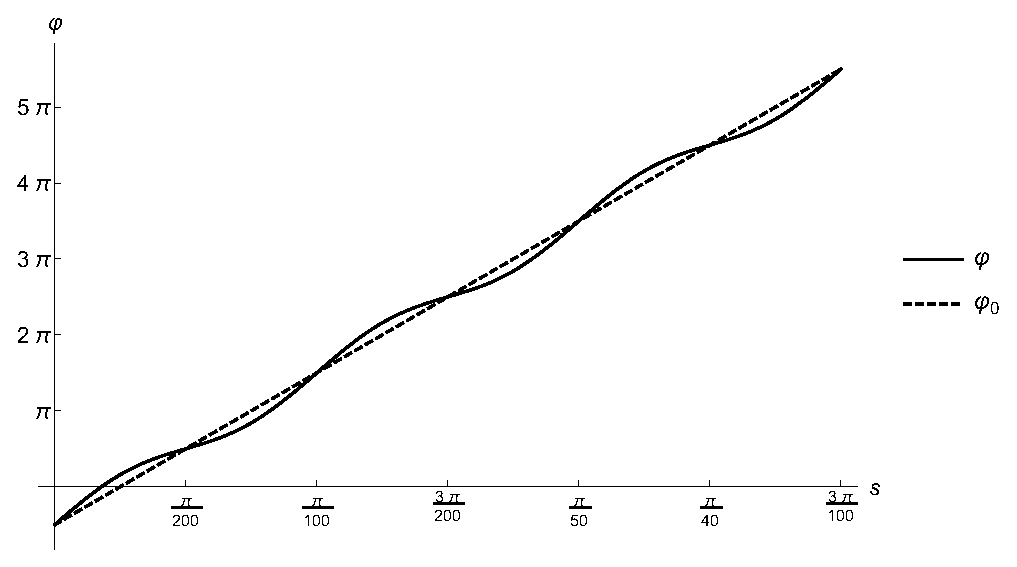
\includegraphics[scale=0.52]{HiperAppA100L2.eps}
\subcaption{Rozwiązanie przybliżone}\label{fig:1a}
\end{minipage}%
\begin{minipage}[b]{.5\linewidth}
\centering
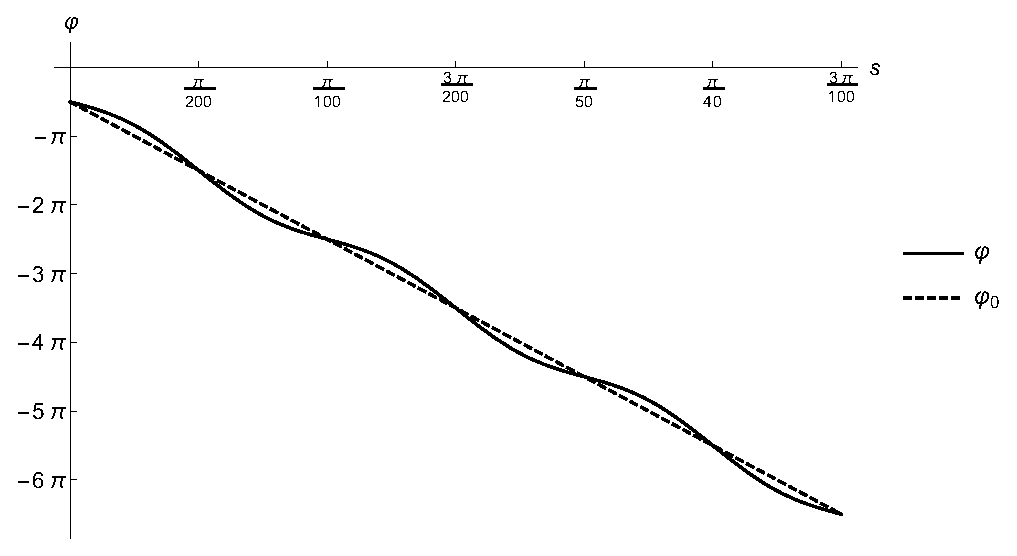
\includegraphics[scale=0.52]{HiperAppA100L2M.eps}
\subcaption{Rozwiązanie przybliżone w odwrotnym działaniu}\label{fig:1b}
\end{minipage}
\begin{minipage}[b]{.5\linewidth}
\centering
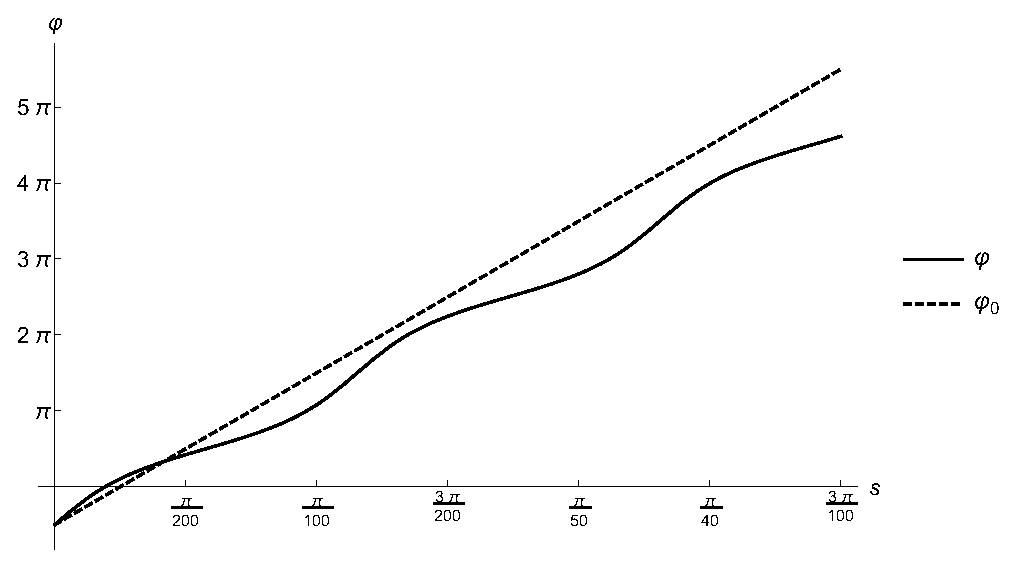
\includegraphics[scale=0.52]{HiperNumA100L2.eps}
\subcaption{Rozwiązanie pełne}\label{fig:1c}
\end{minipage}%
\begin{minipage}[b]{.5\linewidth}
\centering
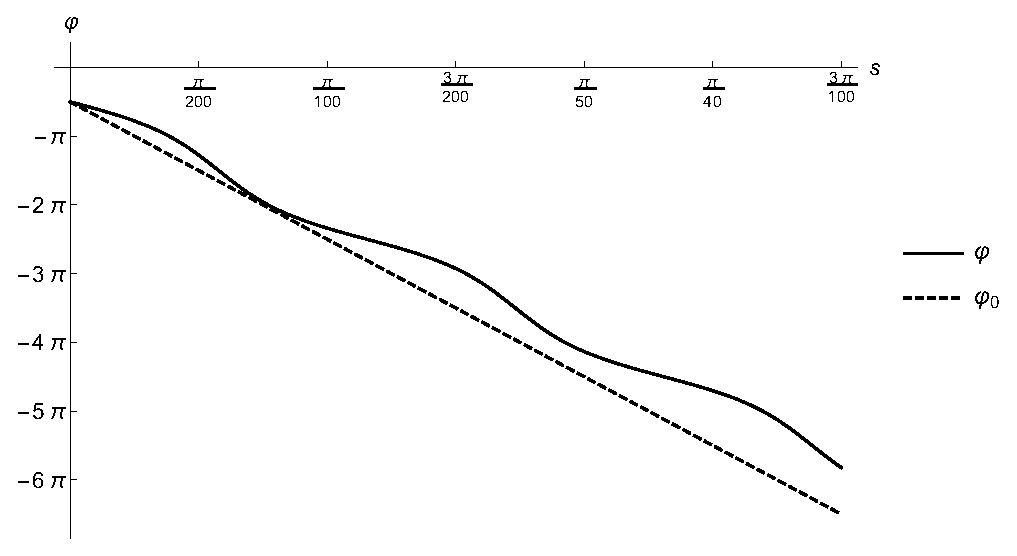
\includegraphics[scale=0.52]{HiperNumA100L2M.eps}
\subcaption{Rozwiązanie pełne w odwrotnym działaniu}\label{fig:1d}
\end{minipage}
\caption{Faza zegara $\varphi$ w ruchu hiperbolicznym dla 
$\ell=0.01$ oraz $\alpha=100$ w porównaniu do fazy 
$\varphi_0$ w układzie bez przyspieszeń. }\label{fig:1}
\end{figure}

\begin{figure}
\begin{minipage}[b]{.5\linewidth}
\centering
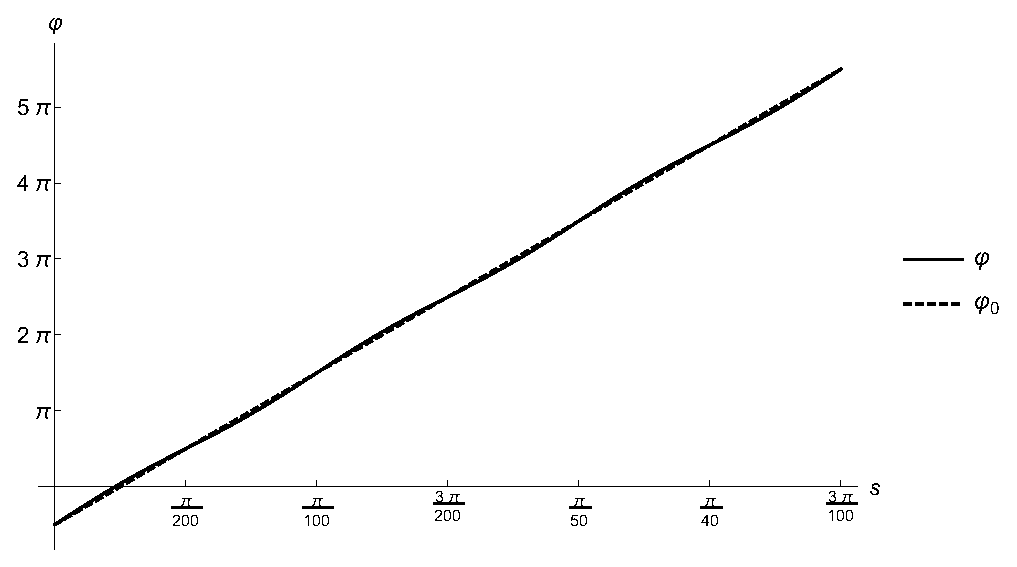
\includegraphics[scale=0.52]{HiperAppA25L2.eps}
\subcaption{Rozwiązanie przybliżone dla $\alpha=25$}\label{fig:2a1}
\end{minipage}%
\begin{minipage}[b]{.5\linewidth}
\centering
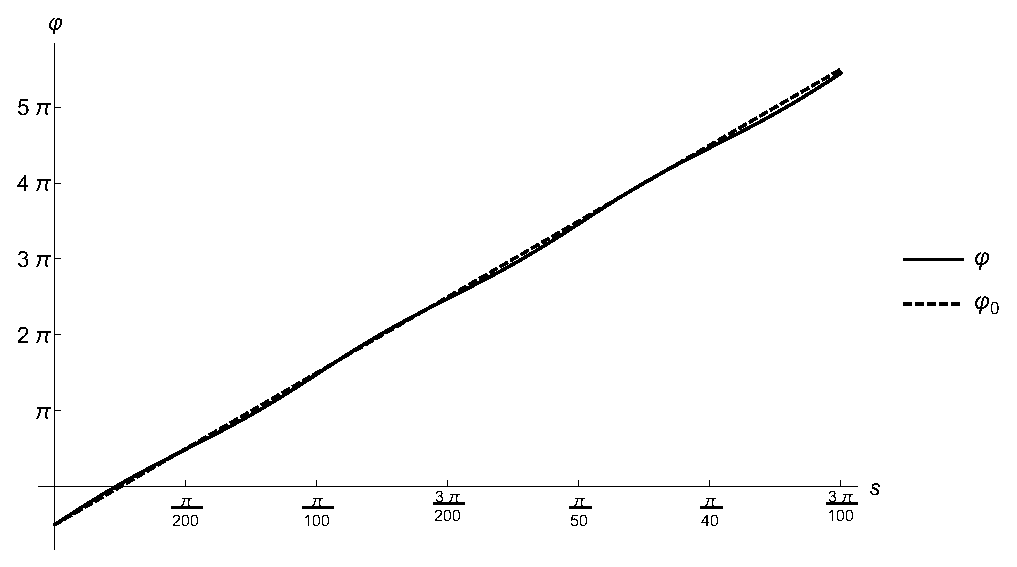
\includegraphics[scale=0.52]{HiperNumA25L2.eps}
\subcaption{Rozwiązanie pełne dla $\alpha=25$}\label{fig:2n1}
\end{minipage}
\begin{minipage}[b]{.5\linewidth}
\centering
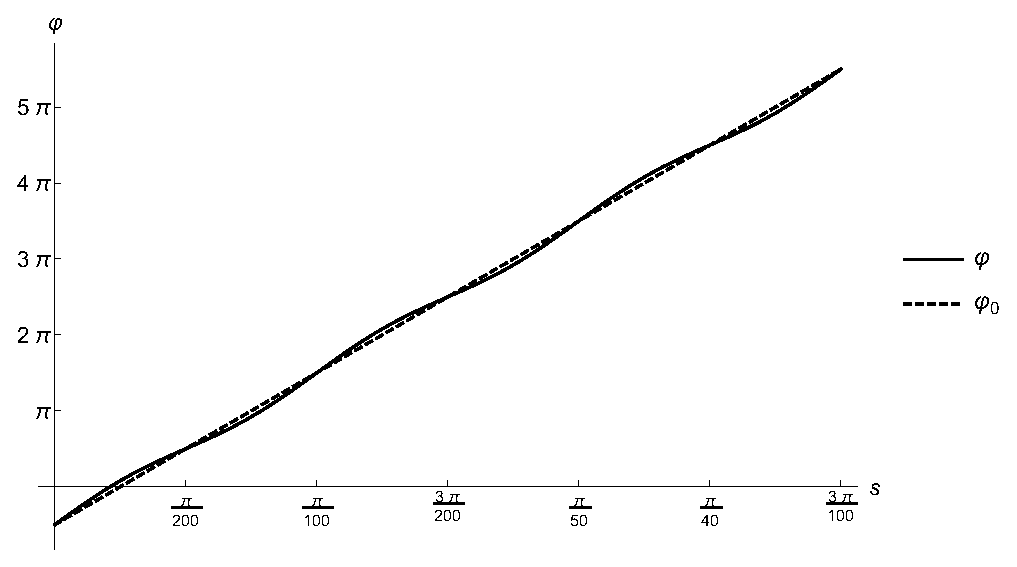
\includegraphics[scale=0.52]{HiperAppA50L2.eps}
\subcaption{Rozwiązanie przybliżone dla $\alpha=50$}\label{fig:2a2}
\end{minipage}%
\begin{minipage}[b]{.5\linewidth}
\centering
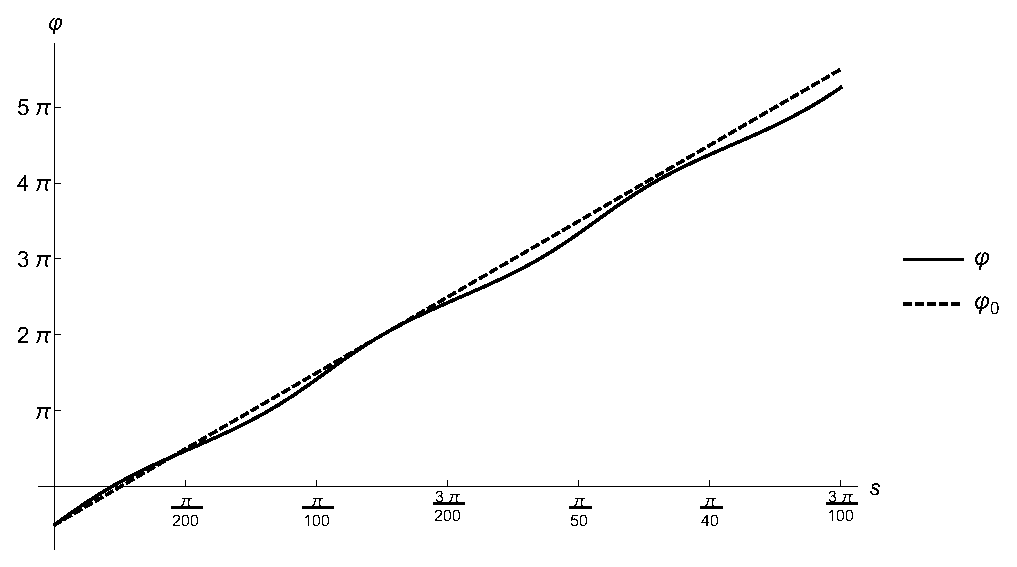
\includegraphics[scale=0.52]{HiperNumA50L2.eps}
\subcaption{Rozwiązanie pełne dla $\alpha=50$}\label{fig:2n2}
\end{minipage}
\begin{minipage}[b]{.5\linewidth}
\centering
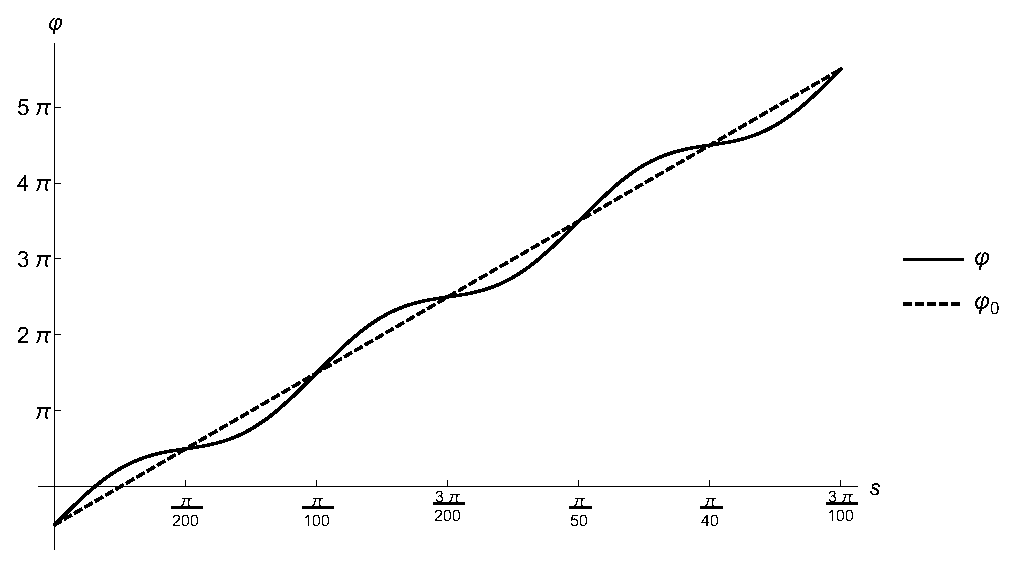
\includegraphics[scale=0.52]{HiperAppA150L2.eps}
\subcaption{Rozwiązanie przybliżone dla $\alpha=150$}\label{fig:2a3}
\end{minipage}%
\begin{minipage}[b]{.5\linewidth}
\centering
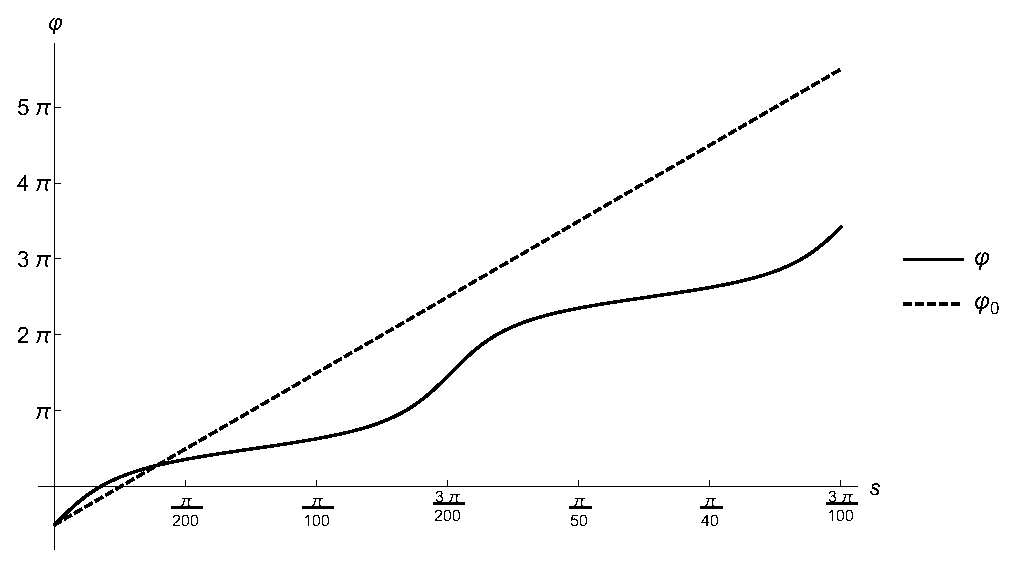
\includegraphics[scale=0.52]{HiperNumA150L2.eps}
\subcaption{Rozwiązanie pełne dla $\alpha=150$}\label{fig:2n3}
\end{minipage}
\caption{Porównanie rozwiązania przybliżonego z rozwiązaniem pełnym
dla faza zegara $\varphi$ w ruchu hiperbolicznym przy
$\ell=0.01$. Linią przerywaną zaznaczono fazę 
$\varphi_0$ w układzie bez przyspieszeń. }\label{fig:2}
\end{figure}


\subsection{Ruch po okręgu}
W przypadku ruchu po okręgu o promieniu $R$ z 
częstością $\omega$ mamy
$\chi = \omega \gamma^2 s$ oraz 
$\alpha = R\omega^2\gamma^2 $.
W takim przypadku faza $\varphi$ jest 
równa~\eqref{phi_wynik_okrag}, a 
przybliżenie dla małych przyspieszeń dane 
przez~\eqref{phi_szereg_okrag}.
\begin{align}\label{phi_wynik_okrag}
\varphi = \omega\gamma^2 s +  
2\text{arctg} \left( 
\sqrt{ 1-\frac{R^2\omega^4\gamma^4}{\left( \pm \frac{2}{\ell} 
-\omega\gamma^2 \right)^2 } }
\text{tg} \left( 
\left( \pm \frac{2}{\ell} -\omega\gamma^2 \right)
\sqrt{ 1-\frac{R^2\omega^4\gamma^4}{\left( \pm \frac{2}{\ell} 
-\omega\gamma^2 \right)^2 } }(s + s_0)/2
\right)  
- \frac{R \omega^2 \gamma^2}{\pm \frac{2}{\ell} -\omega\gamma^2}
\right)
\end{align}
\begin{align*}
s_0 & = \frac{2}{\pm \frac{2}{\ell} -\omega\gamma^2} 
\text{arctg}  
\left( \left( \frac{R \omega^2 \gamma^2}{\pm \frac{2}{\ell} 
-\omega\gamma^2} - 1 \right) \Big /  
\sqrt{ 1-\frac{R^2\omega^4\gamma^4}{\left( \pm \frac{2}{\ell} 
-\omega\gamma^2 \right)^2 } }
\right)\Big /   
\sqrt{ 1-\frac{R^2\omega^4\gamma^4}{\left( \pm \frac{2}{\ell} 
-\omega\gamma^2 \right)^2 } },
\end{align*}
\begin{align}\label{phi_szereg_okrag}
\varphi =  \pm \frac{2}{\ell}s - \frac{\pi}{2} 
+
\frac{R \omega^2 \gamma^2}{\pm 2/\ell - \omega\gamma^2}
\sin ( (\pm 2/\ell - \omega\gamma^2) s )  
+O(\alpha^2).
\end{align}
\begin{figure}
\begin{minipage}[b]{.5\linewidth}
\centering
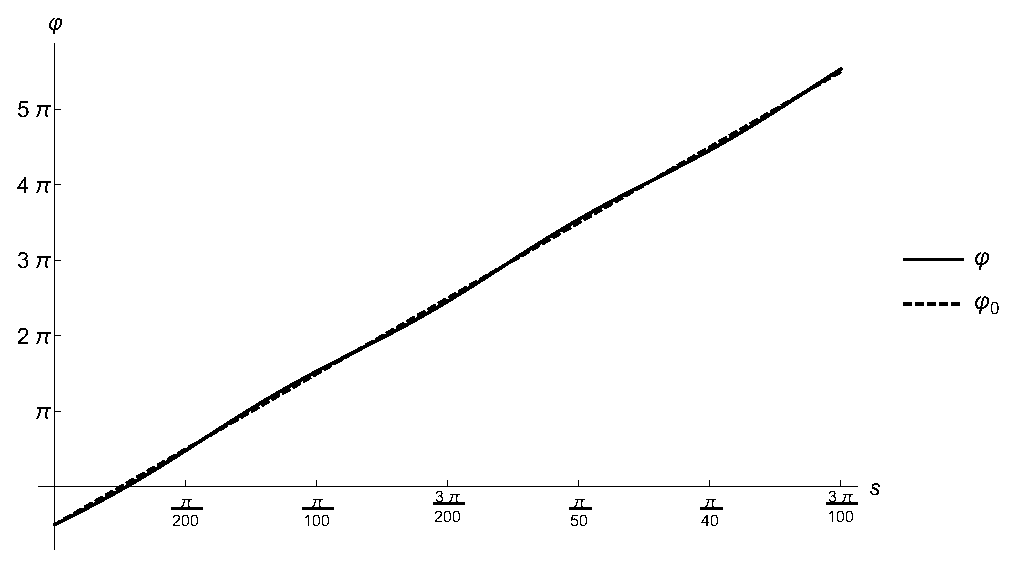
\includegraphics[scale=0.52]{RAppW98R1L2.eps}
\subcaption{Rozwiązanie przybliżone dla $\omega=0,98$}\label{fig:3a1}
\end{minipage}%
\begin{minipage}[b]{.5\linewidth}
\centering
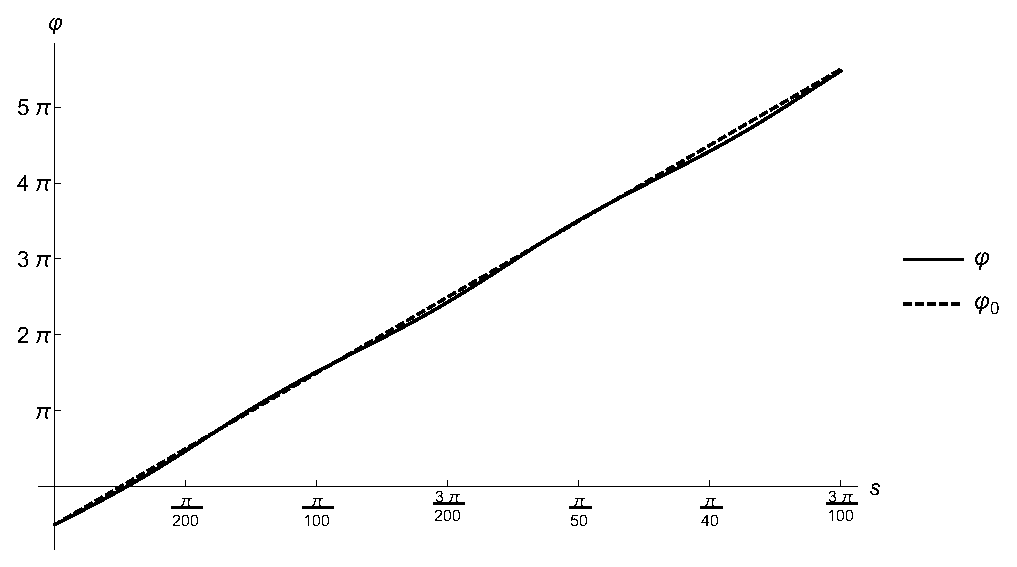
\includegraphics[scale=0.52]{RNumW98R1L2.eps}
\subcaption{Rozwiązanie pełne dla $\omega=0,98$}\label{fig:3n1}
\end{minipage}
\begin{minipage}[b]{.5\linewidth}
\centering
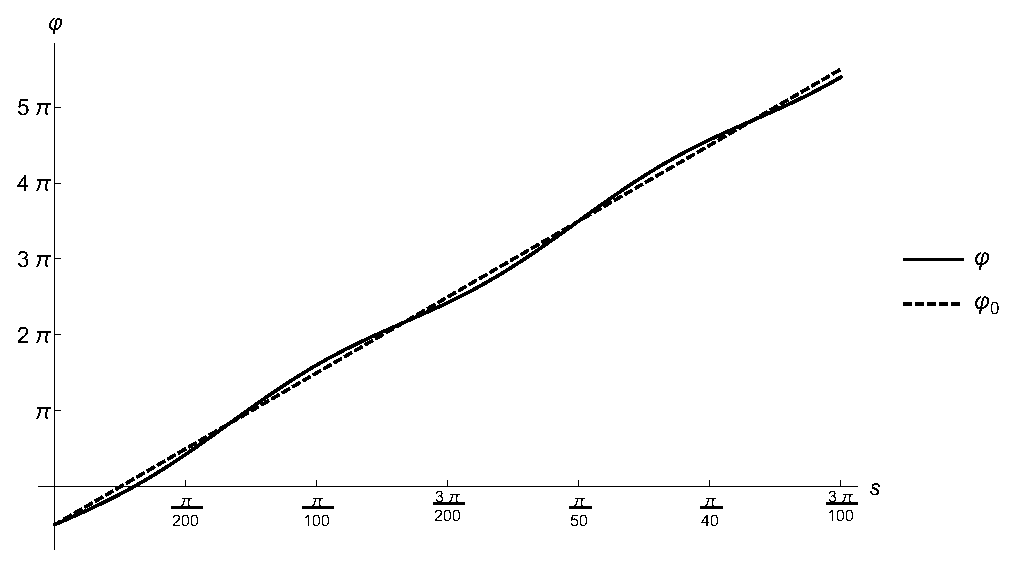
\includegraphics[scale=0.52]{RAppW99R1L2.eps}
\subcaption{Rozwiązanie przybliżone dla $\omega=0,99$}\label{fig:3a2}
\end{minipage}%
\begin{minipage}[b]{.5\linewidth}
\centering
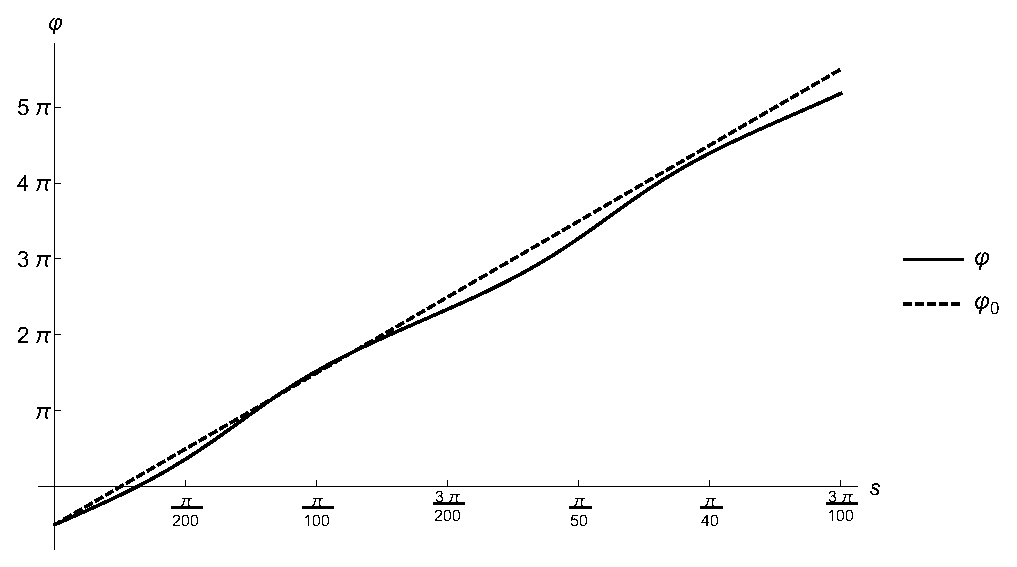
\includegraphics[scale=0.52]{RNumW99R1L2.eps}
\subcaption{Rozwiązanie pełne dla $\omega=0,99$}\label{fig:3n2}
\end{minipage}
\begin{minipage}[b]{.5\linewidth}
\centering
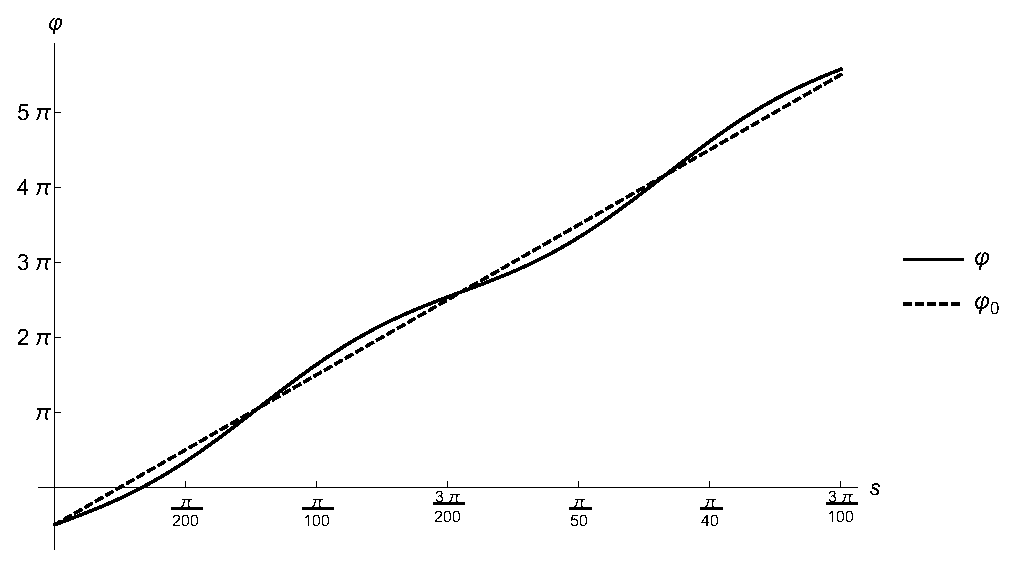
\includegraphics[scale=0.52]{RAppW993R1L2.eps}
\subcaption{Rozwiązanie przybliżone dla $\omega=0,993$}\label{fig:3a3}
\end{minipage}%
\begin{minipage}[b]{.5\linewidth}
\centering
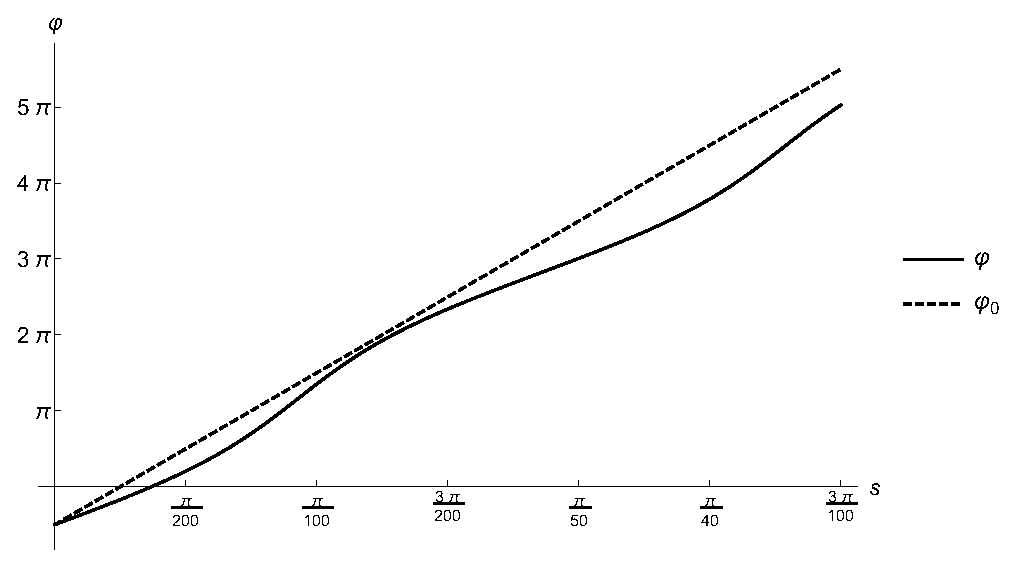
\includegraphics[scale=0.52]{RNumW993R1L2.eps}
\subcaption{Rozwiązanie pełne dla $\omega=0,993$}\label{fig:3n3}
\end{minipage}
\caption{Porównanie rozwiązania przybliżonego z rozwiązaniem pełnym
dla faza zegara $\varphi$ w ruchu po okręgu przy
$\ell=0.01$ i $R=1$ dla różnych prędkości $\omega$. 
Linią przerywaną zaznaczono fazę 
$\varphi_0$ w układzie bez przyspieszeń.}\label{fig:3}
\end{figure}
\newpage
\subsection{Analiza modelu pod kątem pomiaru}
Najprostszym obiektem, dla którego można użyć tego modelu wydaje się
być elektron. Wiemy, że dla małych przyspieszeń hipoteza zegara
wydaje się być spełniona~\cite{}. W tej części oszacujemy rząd 
wielkości przyspieszenia dla którego spodziewamy się 
obserwowalnych odstępstw od hipotezy zegara.
Za $\ell$ możemy podstawić wielkość o wymiarze metra 
charakterystyczną dla elektronu - długość 
Komptonowską fali~\eqref{compton_electron}. 
Wtedy przyspieszenie charakterystyczne dla elektronu 
wynosi~\eqref{ac_electron}.
Dla porównania energie elektronów otrzymywane 
w akceleratorach liniowych są rzędu kilku-kilkunastu GeV.
Dla szacowania przyjmiemy gradient przyspieszenia rzędu
kilku $ \si{\giga\electronvolt \per \metre}$~\cite{Ghotra2015}.
Rząd wielkości przyspieszenia 
szacujemy jako~\eqref{acceleration_electron_nowadays}.
Porównując rzędy wielkości stwierdzamy, że efekty 
raczej nie będą obserwowalne.
\begin{align}\label{compton_electron}
\lambda_e = \approx 2,426 \cdot 10^{-10} \si{\centi\metre}
\end{align}
\begin{align}\label{ac_electron}
\alpha_c \approx 8,244\cdot 10^{9} \si{ \centi\metre^{-1}}
\end{align}
\begin{align}~\label{acceleration_electron_nowadays}
\alpha \approx 10^2 \si{\centi\metre^{-1}}
\end{align}

Komptonowska długość fali protonu wnosi~\eqref{compton_proton}. 
Przyspieszenie charakterystyczne dla protonu wynosi
wynosi~\eqref{ac_proton}.
%$\alpha_c \approx 1,36\cdot 10^{34} 
%\si{\centi\meter^2 \per \second}$.
Energie protonów osiągane w CERN są rzędu 
$7 \si{\tera\electronvolt}$~\cite{CERN}. 
proton doświadczy wtedy przyspieszenia
rzędu~\eqref{proton_acceleration}.
Porównując rzędy wielkości przyspieszeń stwierdzamy, 
że jesteśmy daleko od możliwych obserwacji
\begin{align}\label{compton_proton}
\lambda_p = \approx 1,321 \cdot 10^{-13} \si{\centi\metre}
\end{align}
\begin{align}\label{ac_proton}
\alpha_c \approx 7,57 \cdot 10^{12} \si{ \centi\metre^{-1}}
\end{align}
\begin{align}~\label{proton_acceleration}
\alpha \approx 124  \si{\centi\metre^{-1}}
\end{align}
